\documentclass[12pt]{article}
\renewcommand{\baselinestretch}{2}


\usepackage[a4paper,top=2cm,bottom=2cm,left=2cm,right=2cm,marginparwidth=1.75cm]{geometry}
\usepackage{graphicx}
\usepackage{amssymb}
\usepackage{gensymb}
\DeclareGraphicsExtensions{.pdf,.png}



\title{Structure and dynamics of crystals on a cylinder}
\date{}
\author{}

\begin{document}
\maketitle

 
Two dimensional colloidal crystals are extensively used for understanding important mechanisms of crytallization process, such as nucleation and growth\cite{savage_experimental_2009}, freezing and melting transitions\cite{thorneywork_two-dimensional_2017}\cite{savage_imaging_2006}, and grain boundary dynamics\cite{gokhale_grain_2013}\cite{skinner_supercooled_2011}. Most studies on these mechanisms are based on 2D colloidal crystals grown on flat and unlimited surface. Curved and confined surfaces give rise to additional constraints to the mechanims of crystallization. The effects of Gaussian curvature on crystallization has been demonstrated in colloidal model systems\cite{meng_elastic_2014}\cite{bausch_grain_2003}. Compared to that, the effects of confinement has received less attention. Crystal on the surface of a cylinder provides a good model system to study confinement since a cylinder has zero gaussian curvature, but a finite diameter. This finite size constraint imposes a periodic boundary condition on a maximally packed crystal. The result of this packing constraint was explored theoretically in a system of hard spheres packed inside a cylinder, predicting the appearance of unique structures not present in crystals on flat and unlimited surface\cite{mughal_phyllotactic_2011}\cite{mughal_dense_2012}. These structures have chirality and line-slip defects. The theory was extended to a system of sphere self-assembly on the surface of a cylinder\cite{wood_self-assembly_2013}. Experiments demonstrated sphere packing inside columns using long range attractive interactions resulting in chiral crystals\cite{wu_confined_2017}. Another experiment showed emergence of a line-slip phase when applying forced drainage of wet foams inside a column\cite{winkelmann_simulation_2017}. All these studies contributed in predicting the characteristics of the structure of confined crystals, however, the dynamics remains an unexplored area both theoretically and experimentally. In our work, We implemented a new experimental system where colloidal spheres crystallize on the surface of a cylinder with a short ranged interaction, resembling a hard sphere packing system. This system allowed us perform a comprehensive study on the diverse group of structure emerging from confinement effect and observe the dynamics that come into play.

\begin{figure}[h]
	\setcounter{topnumber}{1}
	\setcounter{bottomnumber}{1}
	\setcounter{totalnumber}{1}
	\renewcommand{\topfraction}{0.95}
	\renewcommand{\bottomfraction}{0.95}
	\renewcommand{\textfraction}{0.15}
	\renewcommand{\floatpagefraction}{0.9}
    \centering
    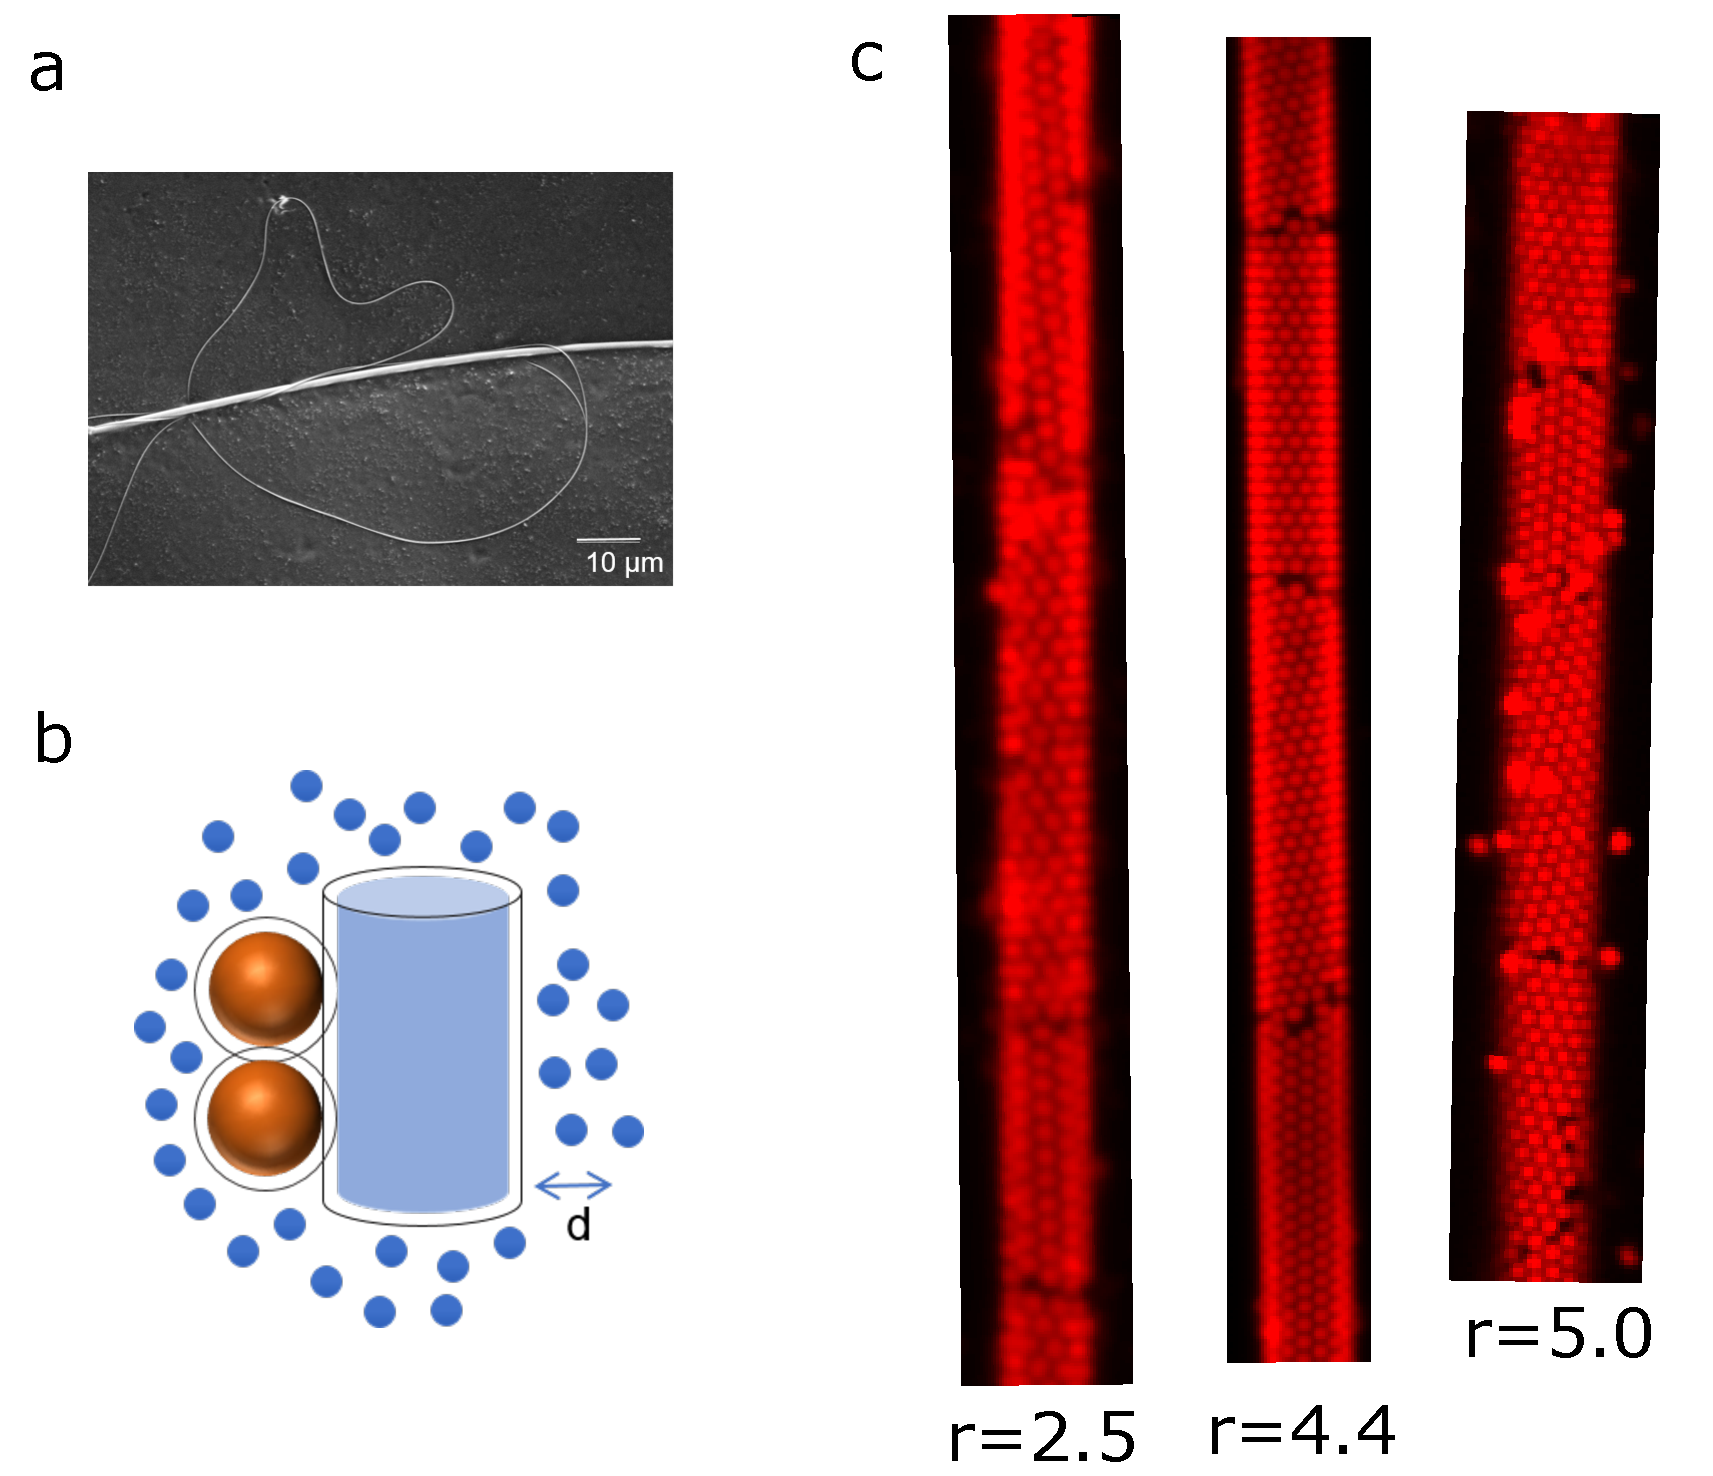
\includegraphics[width = 11.6cm, height = 10cm]{fig1}
    \caption{\textit{(a) SEM image of a tapered optical fiber. Both the thick and thin parts are from the same fiber. A wide range of diameter is accessible using this tapering technique. (b) shows the setup for depletion interaction (c) confocal images of crystals assembled on cylinder for different cylinder to particle size ratios \( r = 2.5\), \( r = 4.4\), \(r = 5.0\).}}
    \label{fig1:setup}
\end{figure}

\paragraph{}

In our experiment, micron sized cylinder is prepared by tapering down an optical fiber using heat and pull method. Colloidal polymer particles with an average diameter of 700 nm are used for crystallization. We mixed the colloidal suspension (0.25\%w/v) with 34 mM Sodium Dodecyl Sulphate (SDS). We put the tapered optical fiber in between two glass cover slips to make the sample chamber, flowed in the mixture of SDS and particles and sealed the chamber. SDS forms micelles with an effective size of about 30 nm that introduce a short-ranged attractive interaction. The interaction range equals to the micelle diameter, about  4.3\% percent of the particle size. Since the potential of depletion interaction increases the overlap of the excluded volume, the force between cylinder and a sphere is stronger than the force between two spheres as long as the cylinder size is larger than the sphere size. As a result, particles form a two-dimensional crystalline layer on the surface of the cylinder. We roughened the surface of the cover slips by coating them with a monolayer of nanoparticles with a size of 300 nm. This roughening prevents the colloidal particles from crystallizing on the cover slips and let them crystallize only on the cylinder surface. We observe the crystals as they grow using a confocal microscope.








\begin{figure}[!ht]
	\setcounter{topnumber}{1}
	\setcounter{bottomnumber}{1}
	\setcounter{totalnumber}{1}
	\renewcommand{\topfraction}{0.95}
	\renewcommand{\bottomfraction}{0.95}
	\renewcommand{\textfraction}{0.15}
	\renewcommand{\floatpagefraction}{0.9}
    \centering
    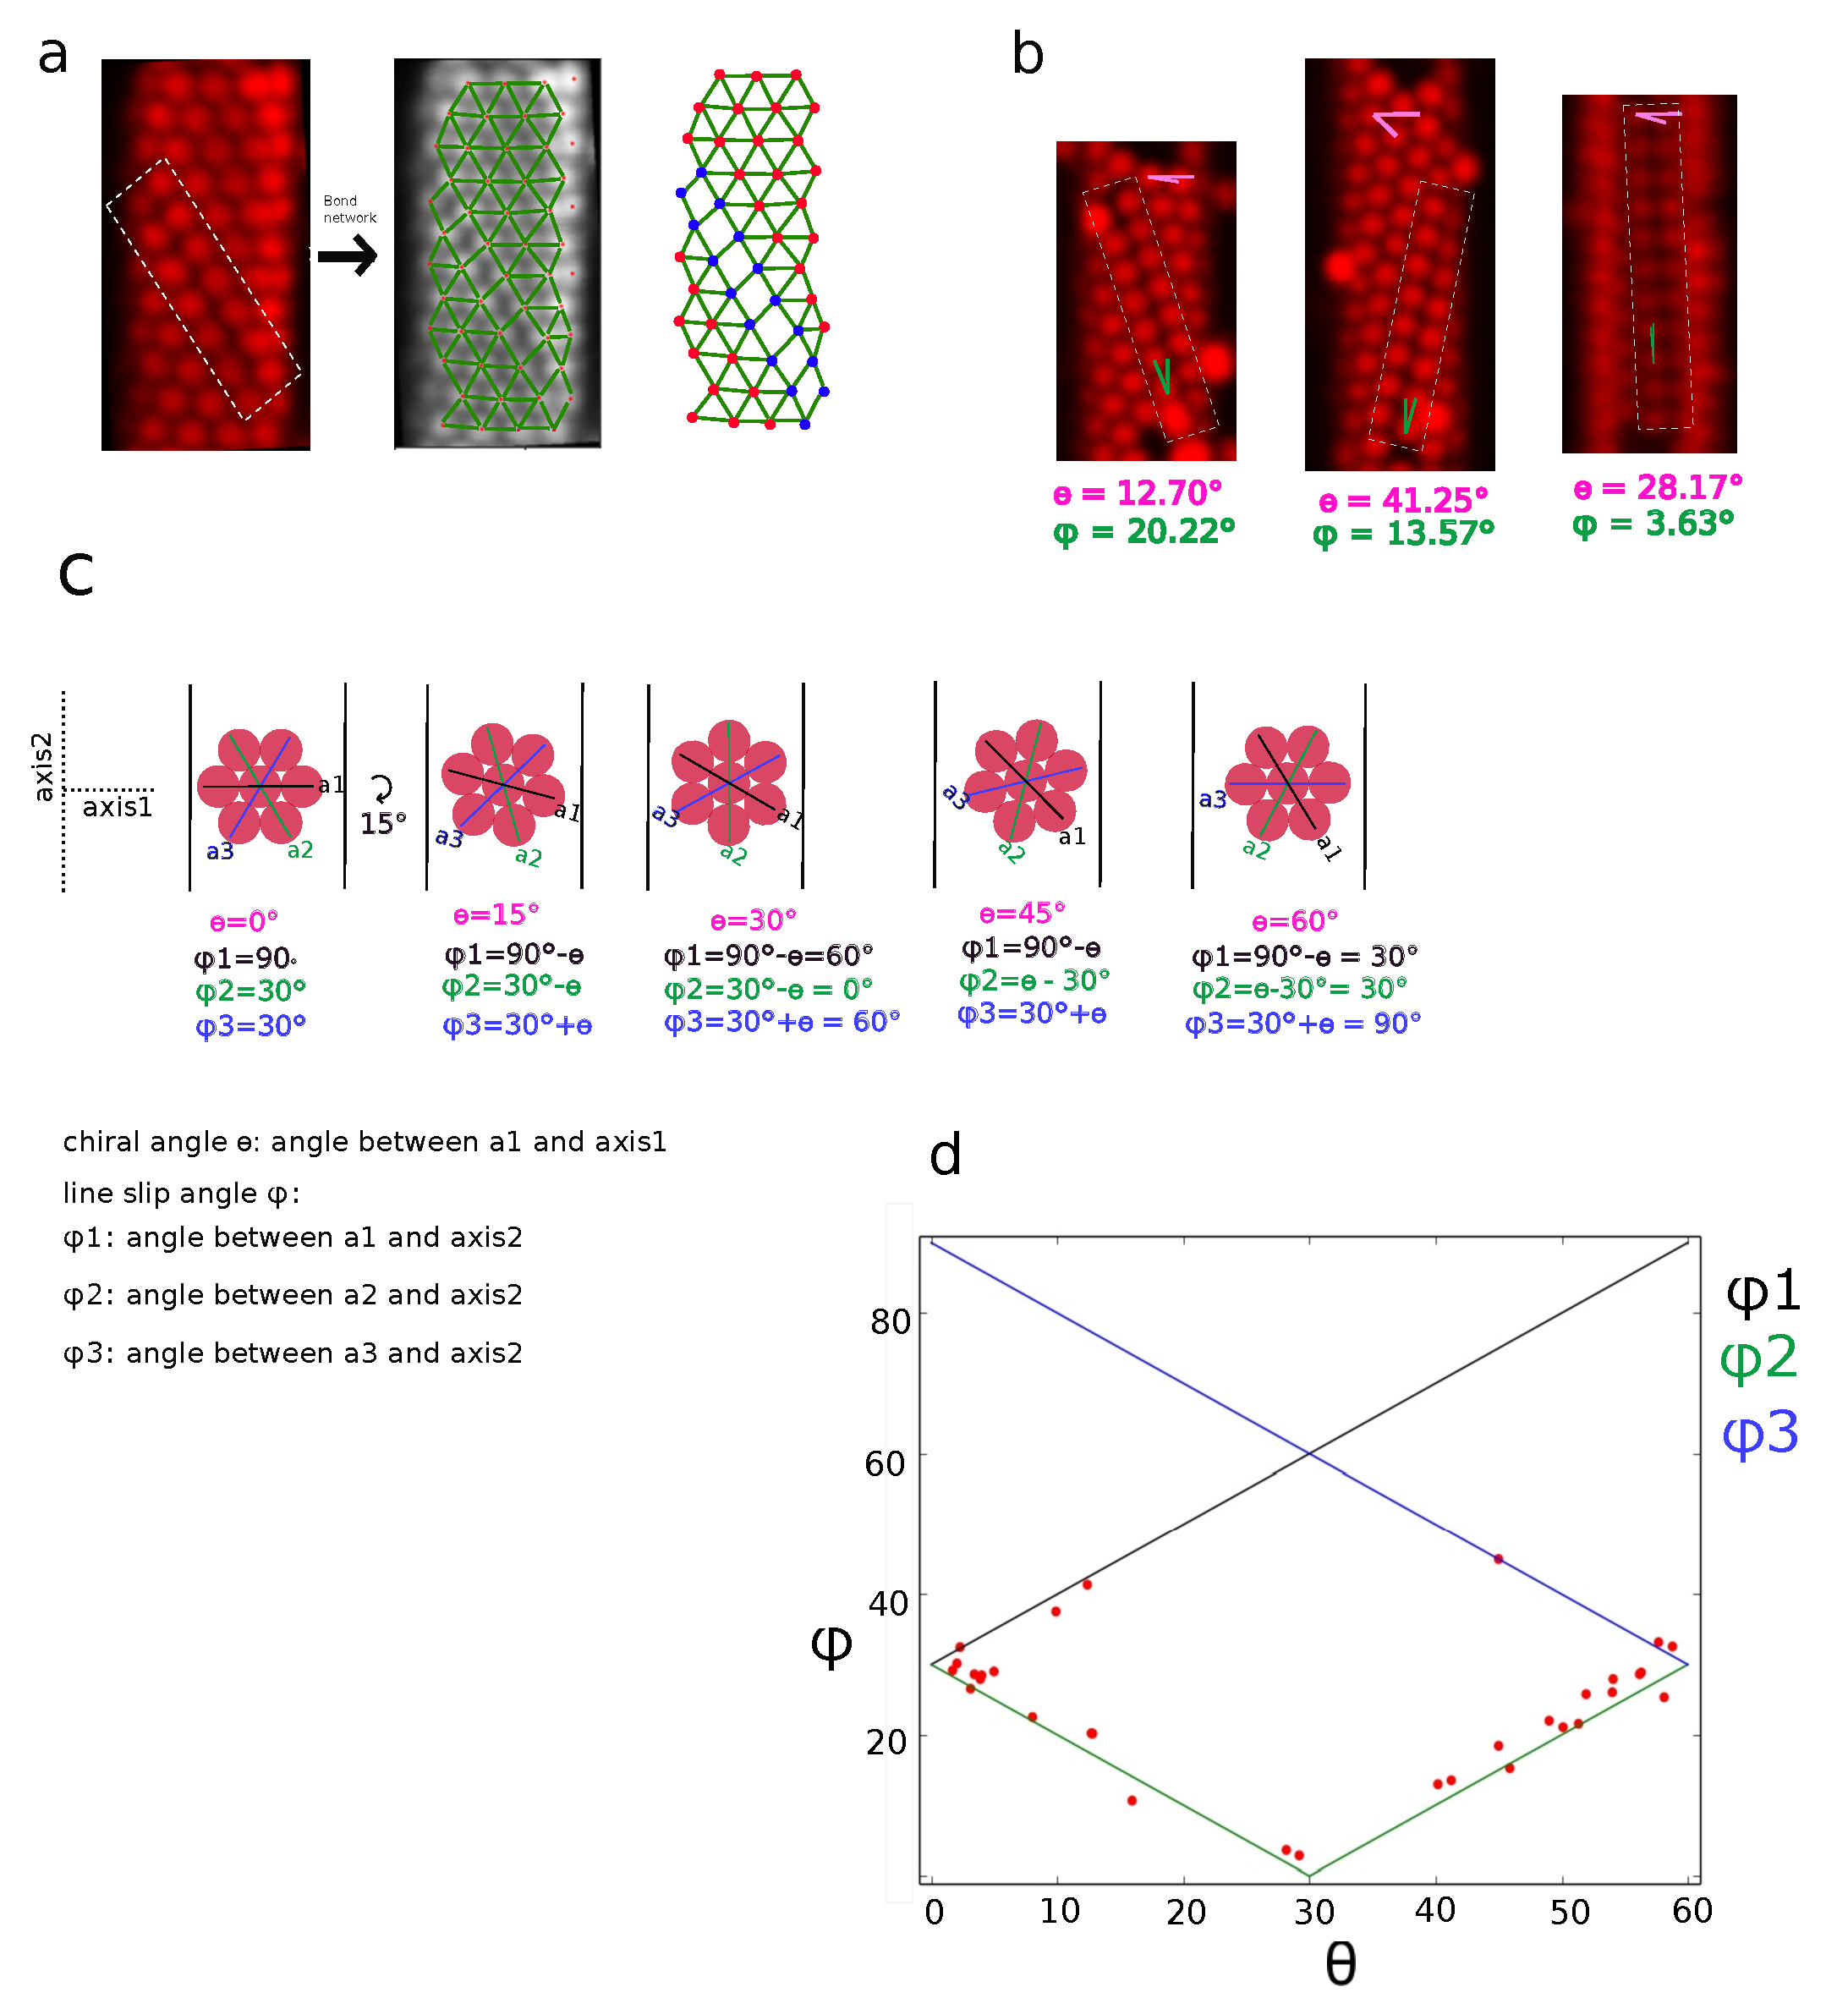
\includegraphics[width = 17cm, height = 18.4cm]{fig2}
    \caption{\textit{(a) line-slip defect is identified by a line of particle pairs with missing contact. The centers of the particles are identified and a bond network is drawn. We can see the line-sip defect consisting blue particles in the bond network. (b) Line-slip structures found in experiment with different $\theta$ and $\phi$ angles. (c) shows how we defined angle $\theta$, $\phi_1$, $\phi_2$, and $\phi_3$. (d) $\theta$ vs $\phi$ plot. The straight lines show theoretical values of $\phi_1$, $\phi_2$, and $\phi_3$. The red data points show experimental values, each point denoting one crystal. Line-slips are more likely to take the angle $\phi_2$.} }
    \label{fig2:line-slips}
\end{figure}

\paragraph{}
Within a few hours, the crystals get wrapped around the cylinder completely and we can observe the unique structures with chirality and line-slip defects. We identified the line-slip defects by watching for a line where triangular symmetry is broken. This line is shown in Fig.\ref{fig2:line-slips}(a), it consists of particle pairs with every particle on the line missing one neighbor. The observation is consistent with the prediction made by Dinsmore et al.\cite{wood_self-assembly_2013}, that line-slip phases are likely to appear for short-ranged interaction. 

\paragraph{}
One interesting aspect of both the crystals and the line-slips is chirality. To understand chirality, we define two angles $\theta$ and $\phi$ . We define chirality of the crystal $\theta$ by the angle between radial axis of the cylinder (axis 1) and one of the lattice vectors \(a_1\). As shown in Fig.\ref{fig2:line-slips}(c), angle $\theta$ can take any value between $0\degree$ and $60\degree$ because of the 6-fold rotational symmetry of the crystal. The line-slip defects can appear along any of the lattice vectors ( \(a_1\),  \(a_2\), and  \(a_3\)).  We define chirality of the line-slip defects $\phi$ by the angle between the corresponding lattice vector and cylinder axis (axis 2). Fig. \ref{fig2:line-slips}(c) shows the possible values of $\phi_1$, $\phi_2$, and $\phi_3$ for different $\theta$ determined by the geometry. 

\paragraph{}
Fig. \ref{fig2:line-slips}(b) shows some crystals observed in experiment with different $\theta$ and $\phi$ values. We identified which of the line-slips are most likely to occur among $\phi_1$, $\phi_2$, and $\phi_3$. This result is shown in Fig. \ref{fig2:line-slips}(d) where line-silp chirality $\phi$ is plotted against $\theta$, each red point corresponds to one crystal found in experiment having chiral angle $\theta$ and line-slip angle $\phi$. We see that most crystals have the lowest line-slip angle $\phi_2$. The crystals prefer having the lowest angle for the line-slips to allow the smallest possible length for the defect line minimizing number of missing contacts as well as free energy. 


\begin{figure}[!ht]
	\setcounter{topnumber}{1}
	\setcounter{bottomnumber}{1}
	\setcounter{totalnumber}{1}
	\renewcommand{\topfraction}{0.95}
	\renewcommand{\bottomfraction}{0.95}
	\renewcommand{\textfraction}{0.15}
	\renewcommand{\floatpagefraction}{0.9}
    \centering
    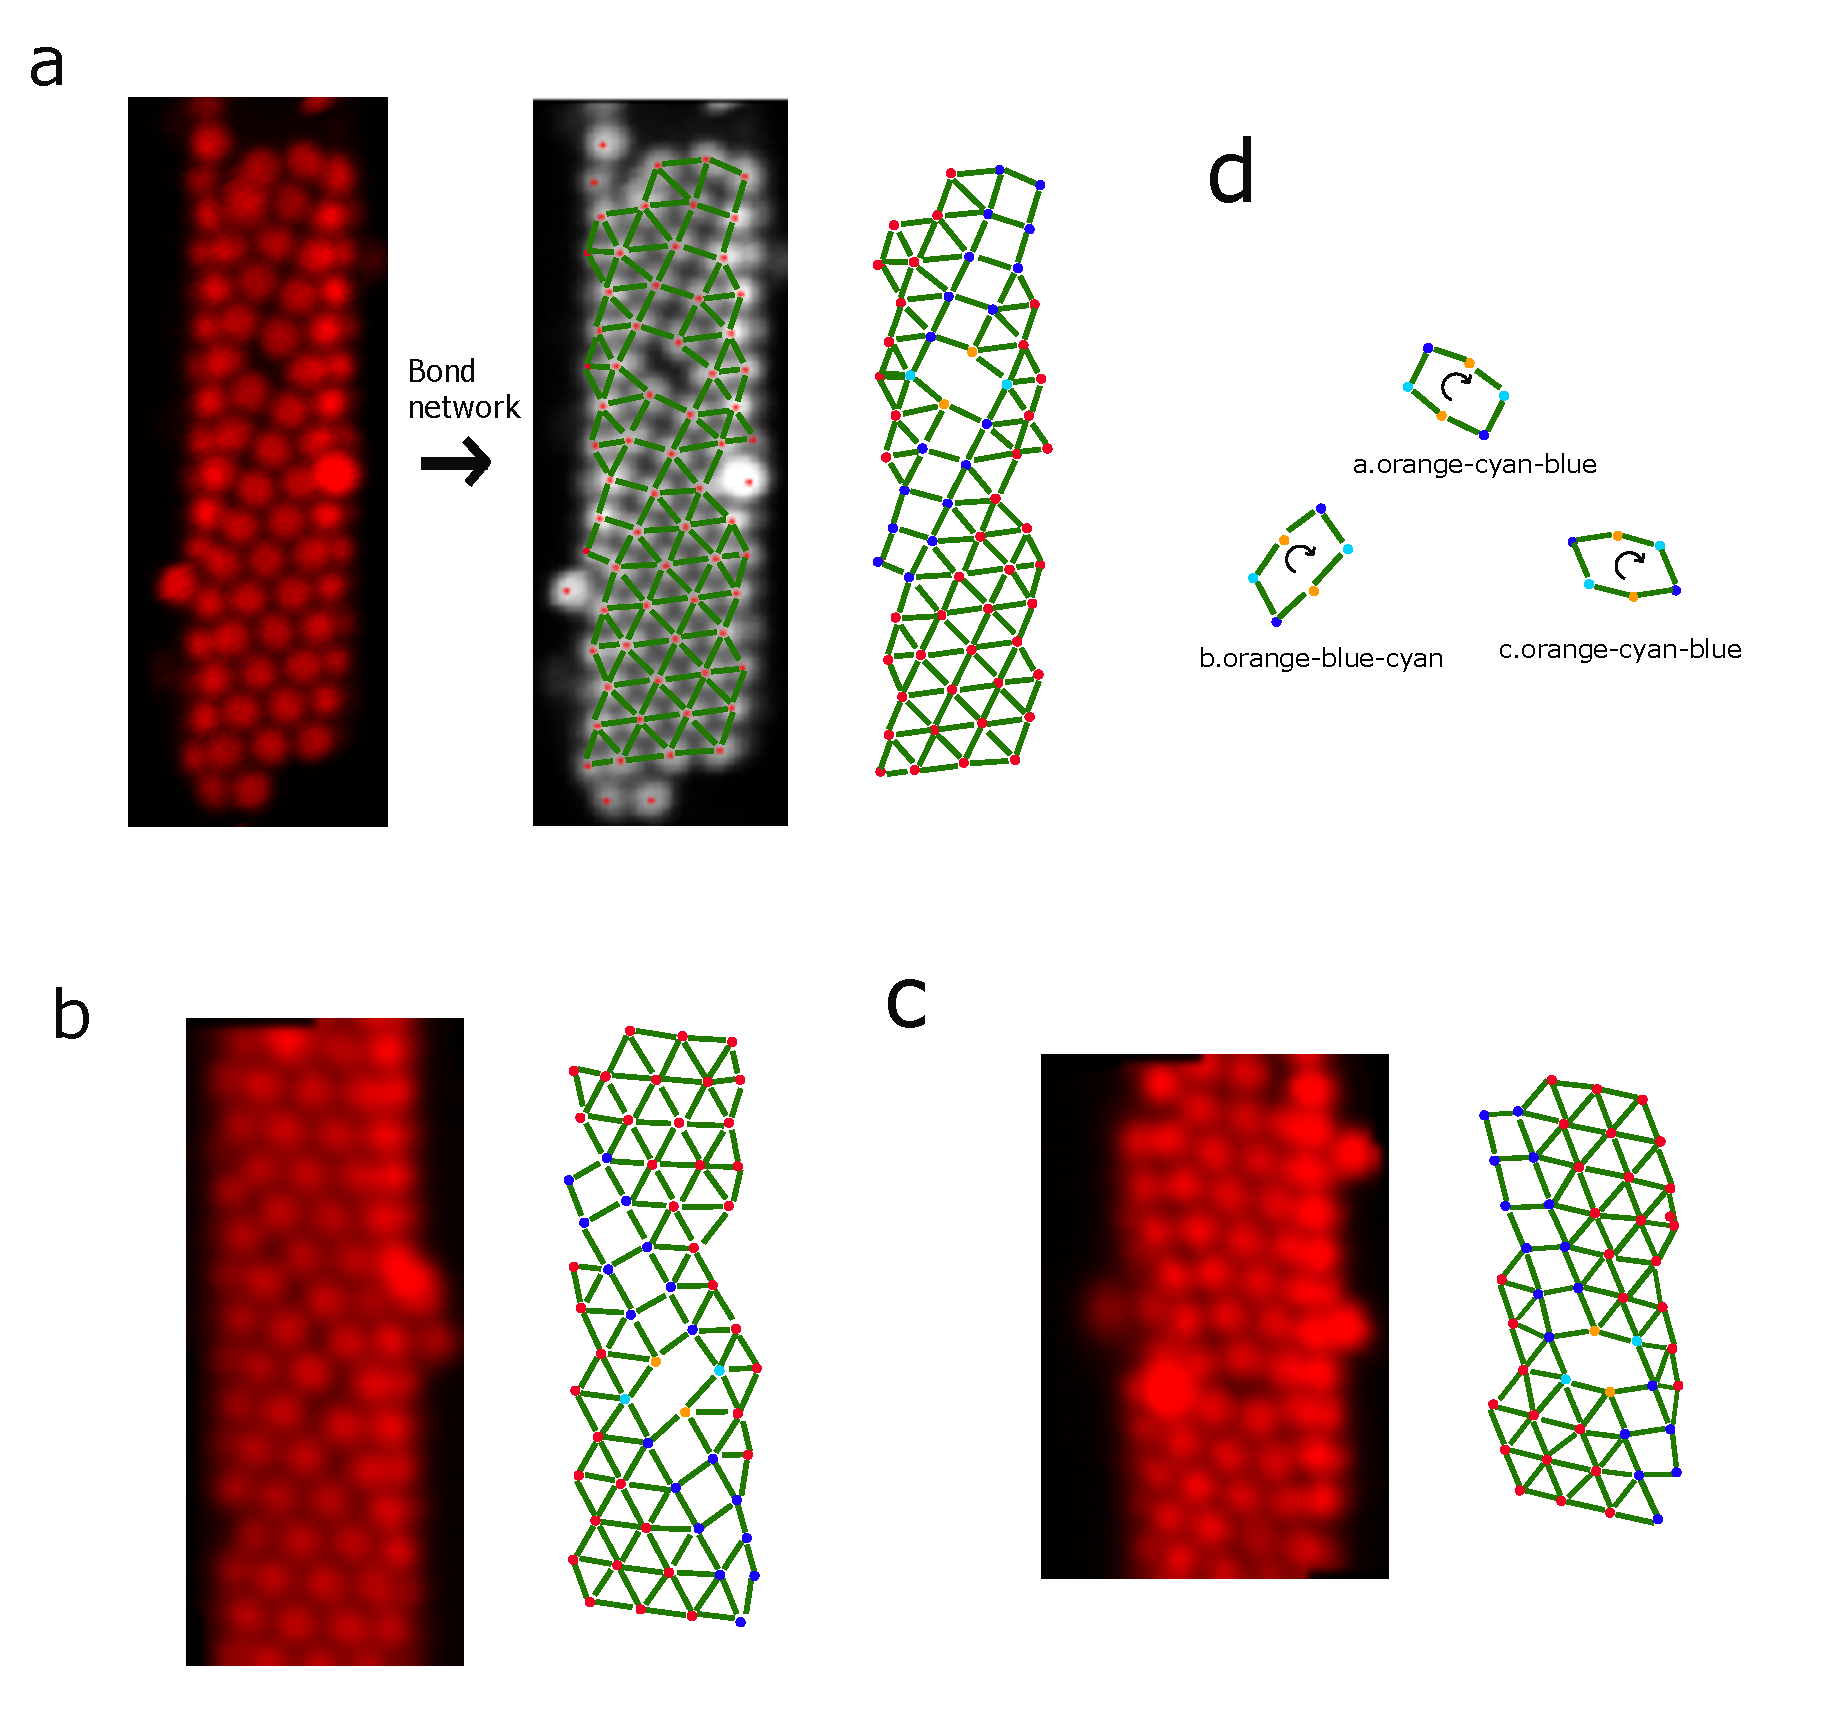
\includegraphics[width = 16.02cm, height = 15cm]{fig3}
    \caption{\textit{(a) A kink in the line-slip is identified from the bond network. The kink is formed by a pair of "blue" particles with 5 bonds each, a pair of "orange" particles with 4 bonds each and a pair of "cyan" particles with 5 bonds each. Even though the number of bonds for blue and cyan particles are the same, symmetry of their bonds is different. All three pairs form a loop that we use to describe a kink. (b) A kink in a line-slip with opposite chirality to the line-slip in (a). (c) A kink forming in the opposite direction to the kink in (b), while the chirality of the line-slip stays same as (b). (d) summary of the kink loops formed in (a), (b), and (c). kink symmetry is influenced both by chirality of line-slips as shown in the difference between (a) and (b), and by the direction of the kink as shown in the difference between (b) and (c).}}
    \label{fig3:kinks}
\end{figure}

\paragraph{}
Besides the conventional line-slips that appear in one straight line and are known to be the ground states, we found a different form of line-slip with a kink in the middle. This is a result of the discontinuity of line slips. As the line-slips are described as a pair of dislocation lines, the newly found geometry can be described as a kink in the dislocation line pair, appearing in a similar way that kinks appear in dislocation lines. Breaking down the structure of a kink as shown in the bond network of Fig. \ref{fig3:kinks}(a), we find two 4-fold particles (orange color), two 5-fold particles (blue color) and two 5-fold particles with different symmetry (cyan color). As all the disclinations position next to each other, there is no net charge.

\paragraph{}
Fig \ref{fig3:kinks}(b) and \ref{fig3:kinks}(c) shows the symmetry breaking that a kinked line-slip can have. (b) shows a kinked line-slip where the line-slip has the opposite handedness to that of (a). As a result, the arrangement of defects at the kink change from orange-cyan-blue (a) to orange-blue-cyan. (c) shows a kinked line-slip where the line-slip has the same handedness as (b). However, as the kink forms in the opposite direction, the arrangement goes back to orange-cyan-blue as shown in (a). Thus we found an additional symmetry breaking that was not present in a straight line-slip. 

\begin{figure}[!ht]
	\setcounter{topnumber}{1}
	\setcounter{bottomnumber}{1}
	\setcounter{totalnumber}{1}
	\renewcommand{\topfraction}{0.95}
	\renewcommand{\bottomfraction}{0.95}
	\renewcommand{\textfraction}{0.15}
	\renewcommand{\floatpagefraction}{0.9}
    \centering
    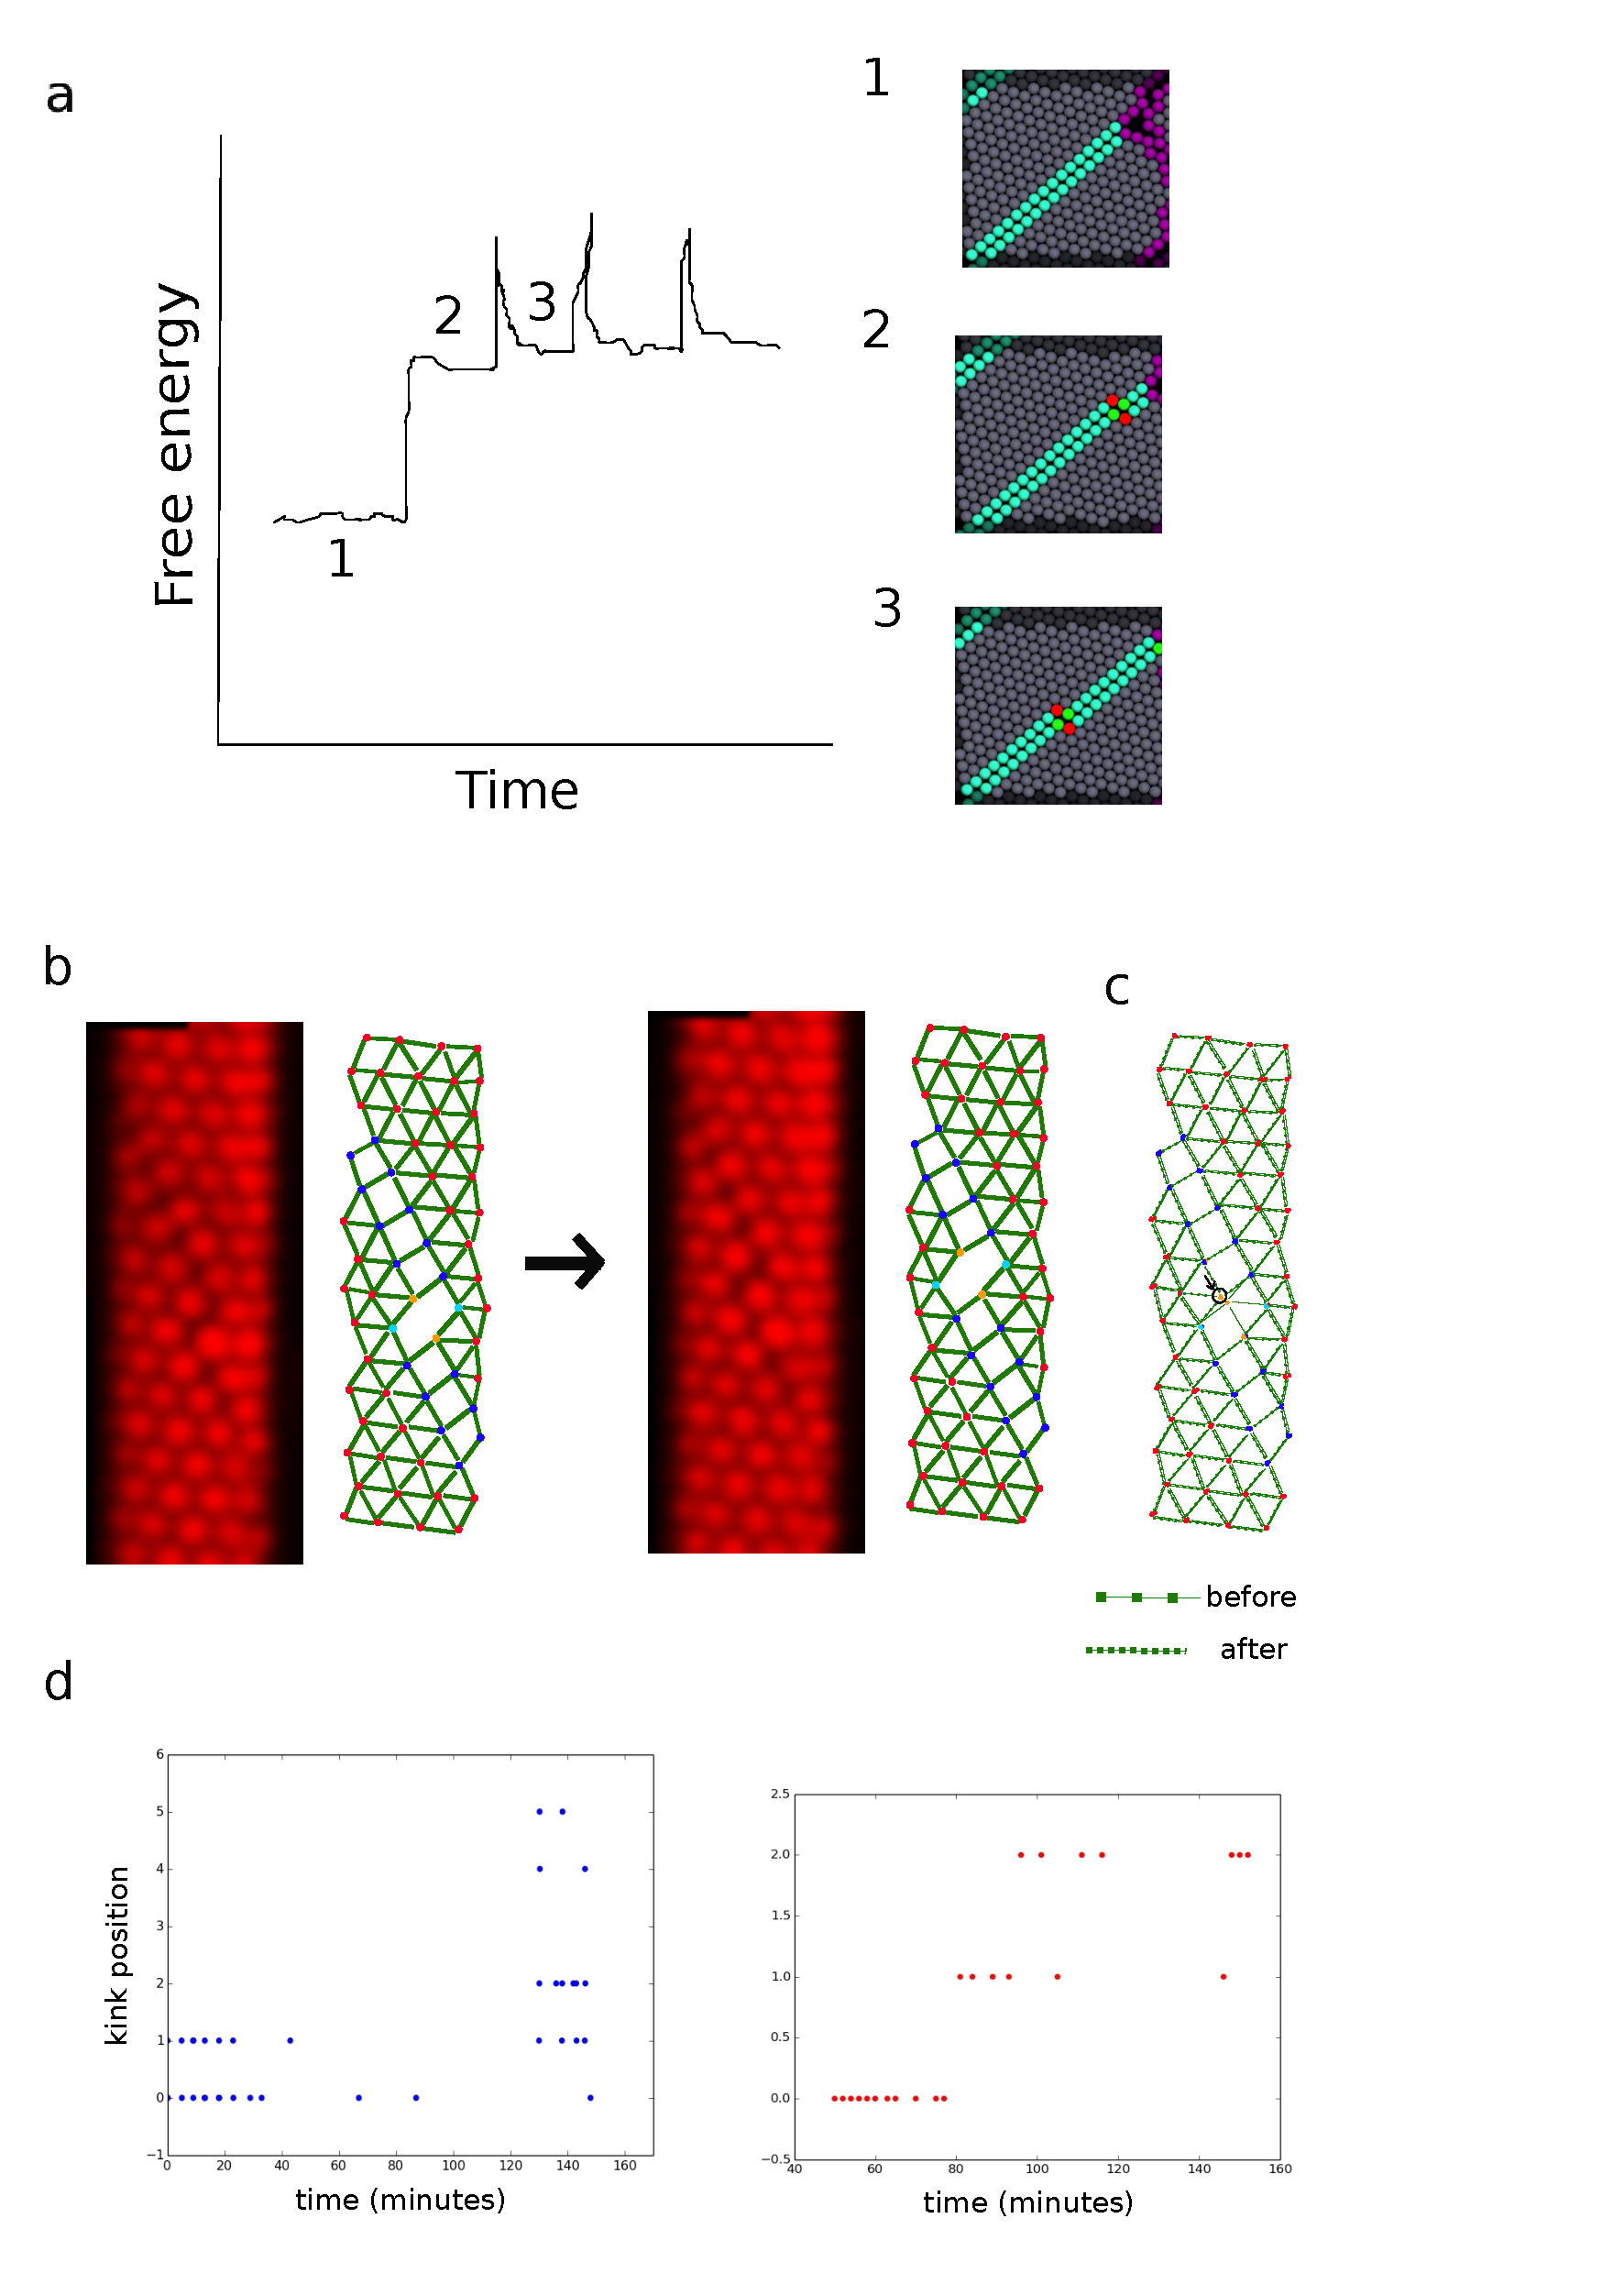
\includegraphics[width = 12cm, height = 16.8cm]{fig4-new}
    \caption{\textit{(a) Calculation of free energy as a function of time when a kink forms, propagates, and disappears. (b) Kink on a line-slip  moving one step in experiment. (c) the bond networks achieved at two different times are overlapped. We see that the orange particle moved downwards, sliding while maintaining the bonds with the two particles left and right. The bonds with the two particles at the top are broken, and two new bonds are formed with two new particles at the bottom. (d) The kink position shown at different times for two different kinks in blue and red data points. }}
    \label{fig4:kink-dynamics}
\end{figure}


\paragraph{}
The kink creates a free space with a volume determined by the structure of the line-slips, smaller than volume occupied by a single vacancy. This fractional vacancy is formed by the stable line-slip defects which are only present on a cylinder, making the kinks unique from a flat space geometry. We performed simulation of crystal growth on a cylinder . (explanation of the simulation). It shows the generation of a kink, how it propagates through the line-slip, and disappears. The free energy of each of these processes is shown in \ref{fig4:kink-dynamics}(a). The energy cost of generating a kink is equivalent to four-bond loss, (? how much kT)less than the energy cost of a vacancy (? in kT), therefore we expect to see them in equilibrium. The kink moves along the line-slip in a one-dimensional track. This movement is achieved by a 4-fold orange particle moving in the opposite direction to the kink movement. In order for the kink to move, a particle breaks two bonds, slide through two bonds and form two new bonds. The energy cost of this process is (? kT). In experiment, we see this kink propagation in \ref{fig4:kink-dynamics}(b) and (c). The kink has moved its position one step closer to the upper end of the crystal. Besides this one-step displacement, we sometimes observe kinks move by sliding multiple particles together (supplementary movie). We have plotted the experimental kink positions with time in \ref{fig4:kink-dynamics}(d). Each integer number marks the position of the kink (or the particle that is responsible for the kink moving), hopping from one integer to another indicates kink taking one step along the line-slip. 



\begin{figure}[!ht]
	\setcounter{topnumber}{1}
	\setcounter{bottomnumber}{1}
	\setcounter{totalnumber}{1}
	\renewcommand{\topfraction}{0.95}
	\renewcommand{\bottomfraction}{0.95}
	\renewcommand{\textfraction}{0.15}
	\renewcommand{\floatpagefraction}{0.9}
    \centering
    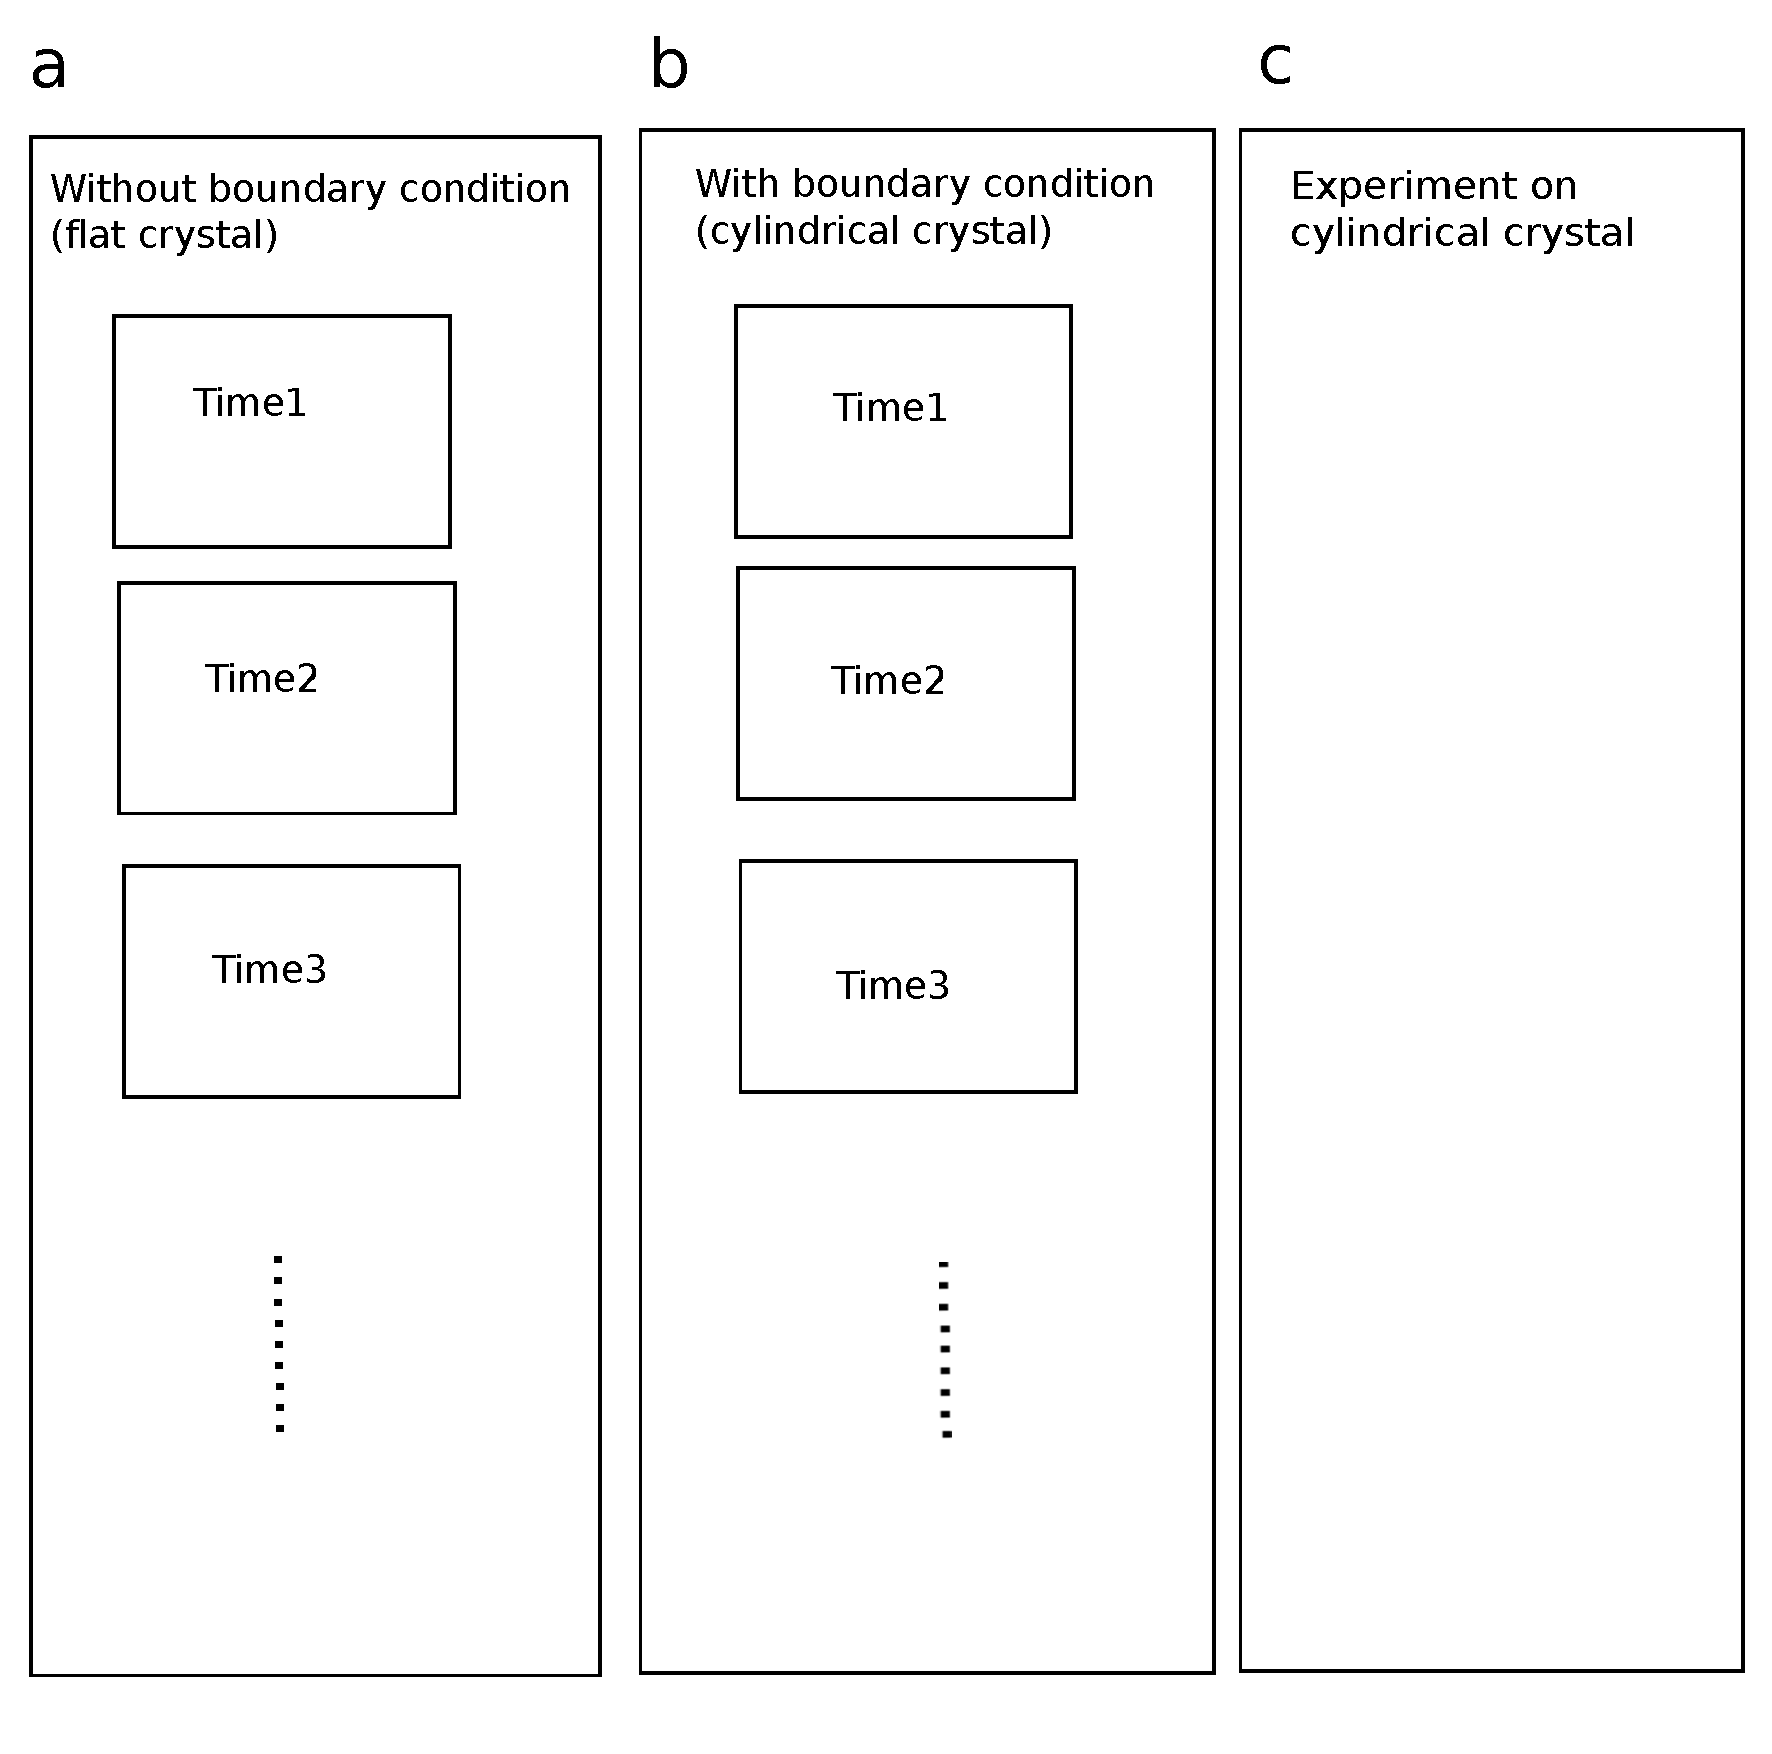
\includegraphics[width = 13cm, height = 13cm]{fig5-new}
    \caption{\textit{ (a) shows simulation of crystal growth on a surface with no periodic boundary condition, representing a flat surface, (b) shows growth on a surface with periodic boundary condition, representing a cylindrical surface. (c) shows how experimental results on crystal growth look like. }
    \label{fig5:cylinder-vs-flat}}
\end{figure}

\paragraph{}

This aspect of the kink dynamics provide additional complexity in the crystallization process. We explored with simulation how crystals form on a cylinder surface and compared it to a flat surface in \ref{fig5:cylinder-vs-flat}(a). We see that as the kinks form, free volume can be trapped inside a crystalline grain. As a result, the coarsening becomes ...(??).


\paragraph{Comments}
Fig 4(a) needed from simulation. Fig 5(a), (b) will show comparison of crystal growth between flat and cylinder surface, without and with periodic boundary condition from simulation. The cylinder diameter should be the same so that the differences between two dynamics become clear. As the kinks and line-slips form, (b) will start showing exotic behaviors- such as volume trapped in kinks, frozen grains, grain boundary fluctuations accelerated by kinks, and so on. (c) will show the similar aspects achieved from experiment. 

\newpage

\bibliography{draft}
\bibliographystyle{unsrt}


\paragraph{Extra figure, does not connect to story well now}


\begin{figure}[!ht]
	\setcounter{topnumber}{1}
	\setcounter{bottomnumber}{1}
	\setcounter{totalnumber}{1}
	\renewcommand{\topfraction}{0.95}
	\renewcommand{\bottomfraction}{0.95}
	\renewcommand{\textfraction}{0.15}
	\renewcommand{\floatpagefraction}{0.9}
    \centering
    \includegraphics[width = 9.36cm, height = 8cm]{fig5}
    \caption{\textit{(a) a kink on the line-slip disappears and turns into a straight line-slip. It is achieved by the upward movement of the kink (or downward movement of two particles) until the kink reaches the grain boundary. (b) bond networks are overlapped. We can see the position changed for two particles, moving the grain boundary downward. (c) A vacancy on a straight line-slip defect helps the line-slip to create a kink. (d)  By overlapping the bond network, we see two particles moving downward, decreasing the free volume of a full vacancy and turning it to a fractional vacancy. The line-slip also gets kinked in the process.   }
    \label{fig6:extra}}
\end{figure}

\end{document}
